\section{Architettura di sistema }
\subsection{Modello Architetturale}
Il progetto Vimar GENIALE rappresenta un’applicazione moderna e avanzata per la gestione di conversazioni intelligenti, sviluppata con un’architettura distribuita e tecnologie all’avanguardia. La sua struttura è pensata per garantire flessibilità, scalabilità e manutenibilità nel tempo, integrando diversi componenti che collaborano per offrire un’esperienza fluida ed efficiente.Per la progettazione del software, si possono adottare due diverse strategie architetturali: l’architettura a strati e l’architettura esagonale.
\begin{itemize}
\item \textbf{L’architettura a strati} è paragonabile a un edificio tradizionale, in cui ogni piano rappresenta un livello ben definito e la comunicazione avviene esclusivamente tra piani adiacenti. Solitamente, si suddivide in:

Presentation Layer: l’interfaccia utente che interagisce con gli utenti.
Business Layer: il livello che contiene la logica di business e le regole applicative.
Persistence Layer: lo strato che si occupa della gestione e dell’accesso ai dati.
Questa organizzazione offre una struttura semplice e ben definita, ideale per applicazioni meno complesse e con pochi collegamenti esterni. Tuttavia, nel caso di un progetto che deve gestire molte integrazioni e garantire una forte modularità, questa soluzione può risultare rigida e difficile da modificare senza impattare altri livelli.
\end{itemize}
\begin{itemize}
\item \textbf{L’architettura esagonale}, invece, è pensata per rendere il sistema più flessibile e indipendente dalle sue dipendenze esterne. Immaginiamola come un hub centrale con diverse porte di accesso: il cuore dell’applicazione (core) è isolato e protetto, mentre tutti i servizi esterni, come il database o il motore AI, si collegano attraverso interfacce ben definite, chiamate ports. Queste porte vengono poi implementate concretamente dagli adapters, che gestiscono le interazioni con il mondo esterno.

Un esempio pratico di questa architettura può essere visto come un aeroporto, dove ogni compagnia aerea ha un terminale dedicato, ma tutti condividono la stessa infrastruttura centrale. Questo permette di mantenere un’organizzazione chiara e modulare, evitando che modifiche a un componente possano impattare il resto del sistema.
\end{itemize}

L’\textbf{architettura esagonale} è la scelta ideale per \textbf{ Vimar GENIALE} perché garantisce una maggiore flessibilità e modularità rispetto all’\textbf{architettura a strati}. La sua capacità di isolare le dipendenze esterne, migliorare la testabilità, facilitare la scalabilità e mantenere il codice ben organizzato la rende perfetta per un progetto che integra tecnologie avanzate e che potrebbe evolversi nel tempo.
\begin{figure}[h]
    \centering
    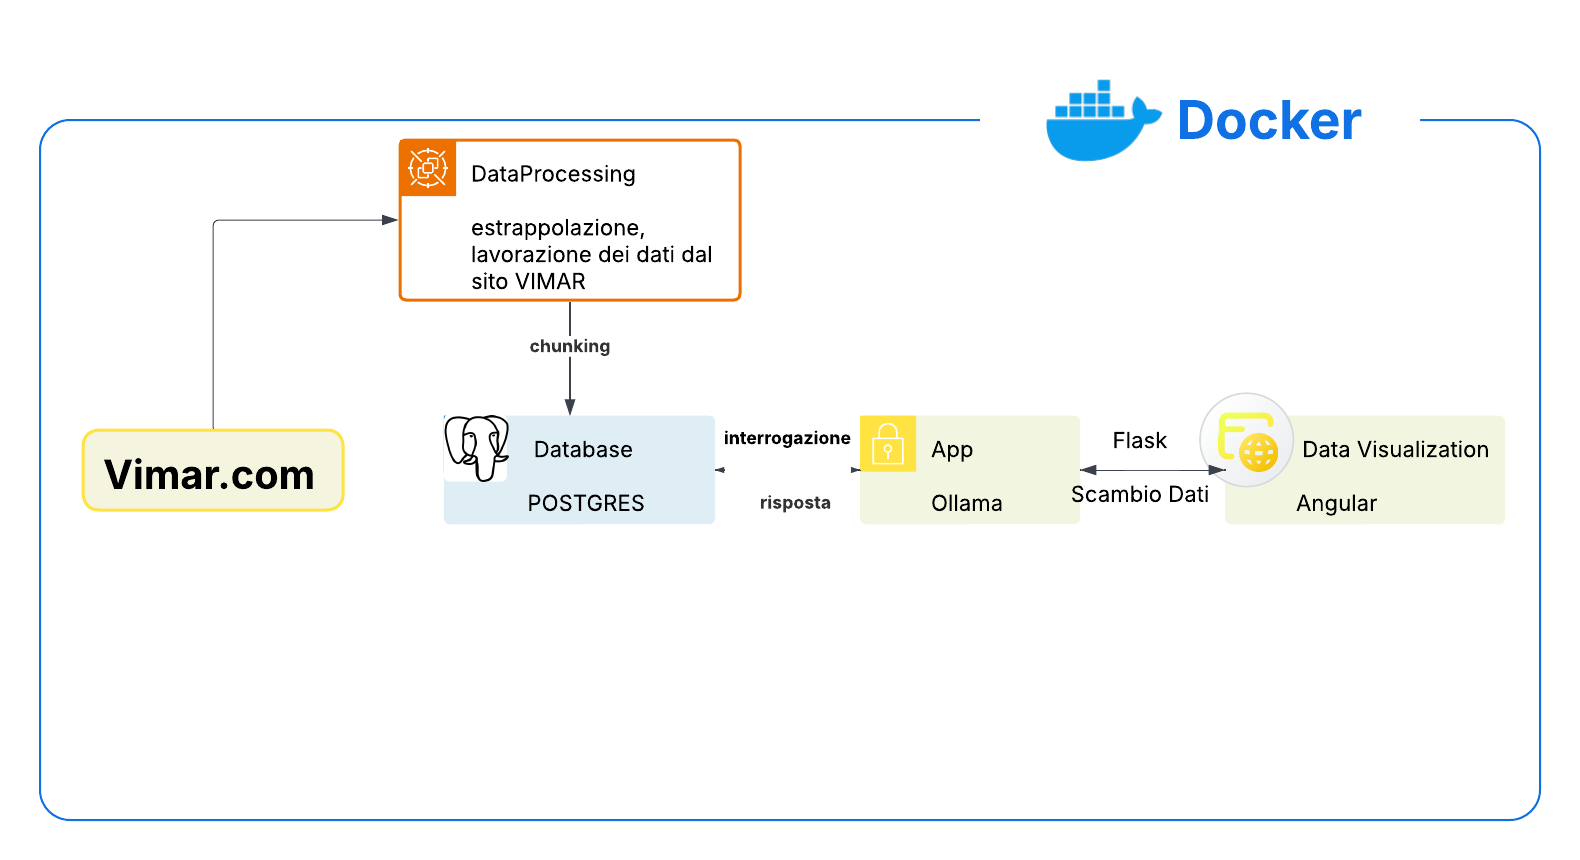
\includegraphics[width=1\textwidth]{Esagonale.png}
\end{figure}